\section{Theoretical Foundation for Anomaly Detection in Sound Classification}
According to the chosen problem-solving approach, our research team will extract sound
features and make predictions following the process shown in the image:

\vspace{-1em}
\begin{figure}[H]
  \centering
  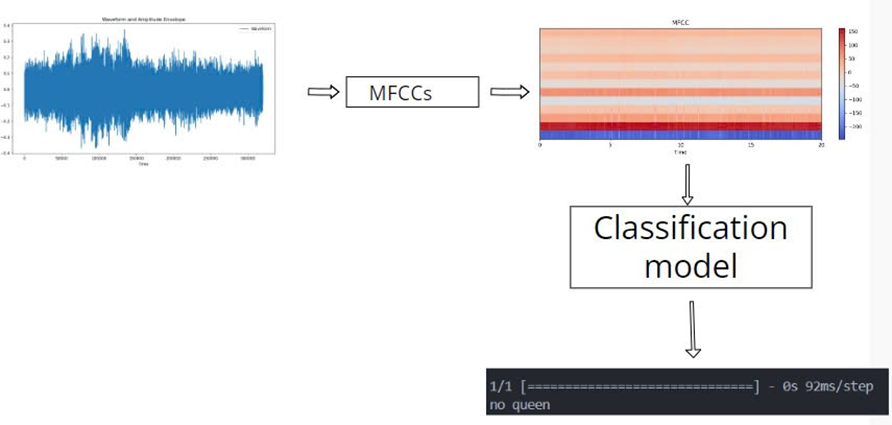
\includegraphics[width=0.47\textwidth]{Audio-Classification-Process.png}
  \caption{Audio Classification Process}
  \label{fig:audio-classification-process}
\end{figure}
\vspace{-1em}

In this process, the audio file will go through the MFCC feature extraction step to
transform from the time domain to the frequency domain. Afterward, the classification
model will output the result indicating whether the audio file contains a queen bee or not.
The two classification models we used are the Convolutional Neural Network (CNN) and the
Long Short-Term Memory (LSTM) combined with CNN (LSTM+CNN).
